\documentclass[12pt]{article}

% #################### PREAMBLE ##########################

% Global margins for the document:
\usepackage[left=0.6cm,
    right=0.6cm,
    bottom=2cm,
    top=2cm,
]{geometry}

% Define spacing between paragraphs in the document:
\setlength{\parindent}{0.5cm} % default indentation before the first line of a paragraph.
\setlength{\topskip}{0.2cm} % indentation at the begging of the first paragraph of every page:
\setlength{\parskip}{0.3cm} % indentation after every paragraph

% Font configurations:
\usepackage{fontspec}
\setmainfont{FreeSerif}

% For justify and some other alignment extensions:
\usepackage{ragged2e}

% Math related packages:
\usepackage{amsmath, amssymb, amsthm}
% For vectors:
\usepackage{esvect}
% Proper calculates where the not line should be drawn:
\usepackage{centernot}
% Theorem definitions:
\newtheorem{thm}{Theorem}
\newtheorem{lem}[thm]{Lemma} % a lemma that shares a counter with the Theorem.
\newtheorem{defn}{Definition}
% Package for system of equations
\usepackage{systeme}

% Embedding *.jpg abd *.png images
\usepackage{graphicx}
\graphicspath{{data/}{../data/}} % define the path to the images

% Provides an underline command which will break over line ends:
\usepackage{ulem}

% Better lines for tables:
\usepackage{hhline}

% Allows enumerate environment to customize the label:
\usepackage{enumitem}

% Multirow :
\usepackage{multirow}

% To use arrays:
\usepackage{array}

% Custom commands for table alignment when dealing with a lot of text (needs array and ragged2e):
\newcolumntype{L}[1]{>{\raggedright\let\newline\\\arraybackslash\hspace{0pt}}m{#1}}
\newcolumntype{C}[1]{>{\centering\let\newline\\\arraybackslash\hspace{0pt}}m{#1}}
\newcolumntype{R}[1]{>{\raggedleft\let\newline\\\arraybackslash\hspace{0pt}}m{#1}}

% Hyper links to places inside the document:
\usepackage{hyperref}
\hypersetup{
    colorlinks=true,
    % These take rgb values as a fraction of n/255.
    % That is really not how RGB works!
    linkcolor=[rgb]{0.1, 0.2, 1},
    filecolor=[rgb]{0.1, 0.2, 1},
    urlcolor=[rgb]{0.1, 0.2, 1},
    citecolor=[rgb]{0.1, 0.2, 1},
    unicode=true,
}
\urlstyle{same}

% For fancy programming code formatting and coloring:
\usepackage{minted}

% For pretty quotes:
\usepackage{epigraph}
\setlength\epigraphwidth{1\textwidth}
\setlength\epigraphrule{0pt}

% For a footer and header:
\usepackage{fancyhdr}
\pagestyle{fancy}

\fancyhead[L]{Top Left Head}
\fancyhead[C]{Center Head}
\fancyhead[R]{Top Right Head}

\fancyfoot[L]{Bottom Left Foot}
\fancyfoot[C]{Page \thepage}
\fancyfoot[R]{Bottom Right Foot}

% Bibliography:
\usepackage{csquotes}
\usepackage[backend=biber]{biblatex}
\addbibresource{init.bib}

% For inserting loremipsum random text:
\usepackage[pangram]{blindtext}

% Allows adding sub tex files to the main tex file:
\usepackage{subfiles} % Best loaded last in the preamble

% #################### DOCUMENT BEGIN ####################

\begin{document}

% Title:
\begin{titlepage}
    \begin{center}
        \Large
        \textbf{Курсова Работа} \\
        Име на предмета Esse deserunt consequat \\
        \vspace*{0.2cm}
        \large
        Име на университет Dolor eu et enim irure voluptate deserunt official \\
        \vspace*{3cm}

        \Large
        Тема: \\
        \huge
        \textbf{Deserunt reprehenderit magna laborum \\ dolor adipisicing in fugiat}

        \vfill

        \large
        Лого на унито:
        \begin{center}
            
\includegraphics[width=0.3\linewidth]{sample.png}
        \end{center}

        \large \vfill
        \today \\
        Пешо Пешев Пешков \\
        Фак. номер: 123456
    \end{center}
\end{titlepage}

\newpage

\begin{center}
    {\Huge Big Centered Text}
\end{center}

1. Tiny noindent text: \\
{\tiny\noindent\Blindtext[1][1]}

2. Scriptsize text with added additional 4cm indentation, which is then removed -4cm:

\addtolength{\parindent}{4cm}
{\scriptsize\Blindtext[1][1]}
\addtolength{\parindent}{-4cm}

3. Footnotesize flush right text:
\begin{flushright}
{\footnotesize Cillum proident aliquip ipsum do do cupidatat laboris. Mollit proident eiusmod adipisicing ad ipsum nulla consectetur esse. Incididunt laboris irure do eu ad dolore ad ea pariatur sint. Eu ea exercitation incididunt excepteur quis.}
\end{flushright}

4. Normalsize flus left text:
\begin{flushleft}
{\normalsize Something. This paragraph contains no information and its purposes is to provide an example on how to insert white spaces and lines breaks. Right here -> \textbackslash\textbackslash \\
When a line break is inserted, the text is not indented, there are a couple of commands for line breaks. \textbackslash newline \newline
This paragraph contains full line break. \textbackslash hfill and \textbackslash break \hfill \break For combining two commands}
\end{flushleft}

5. large centered text:
\begin{center}
{\large Nisi qui culpa pariatur velit deserunt nulla nulla dolor cillum est do nulla ut. Nisi qui culpa pariatur velit deserunt nulla nulla dolor cillum est do nulla ut.}
\end{center}

6. Large text after 2 newlines (baselineskip) : \\[2\baselineskip]

{\Large The environments center, flushleft, flushright, justify should only be used with text paragraphs. They can NOT format other LaTeX objects!}

\newpage

\tableofcontents
\listoffigures
\listoftables
\setcounter{section}{7}

\newpage

\section{Images and figures}

Graphics with set width 0.3 of linewidth: \\
\begin{center}
    
\includegraphics[width=0.3\linewidth]{sample.png}
\end{center}

\noindent LaTeX includegraphics wrapped in a figure: \\
\begin{figure}[ht!]
    \centering
    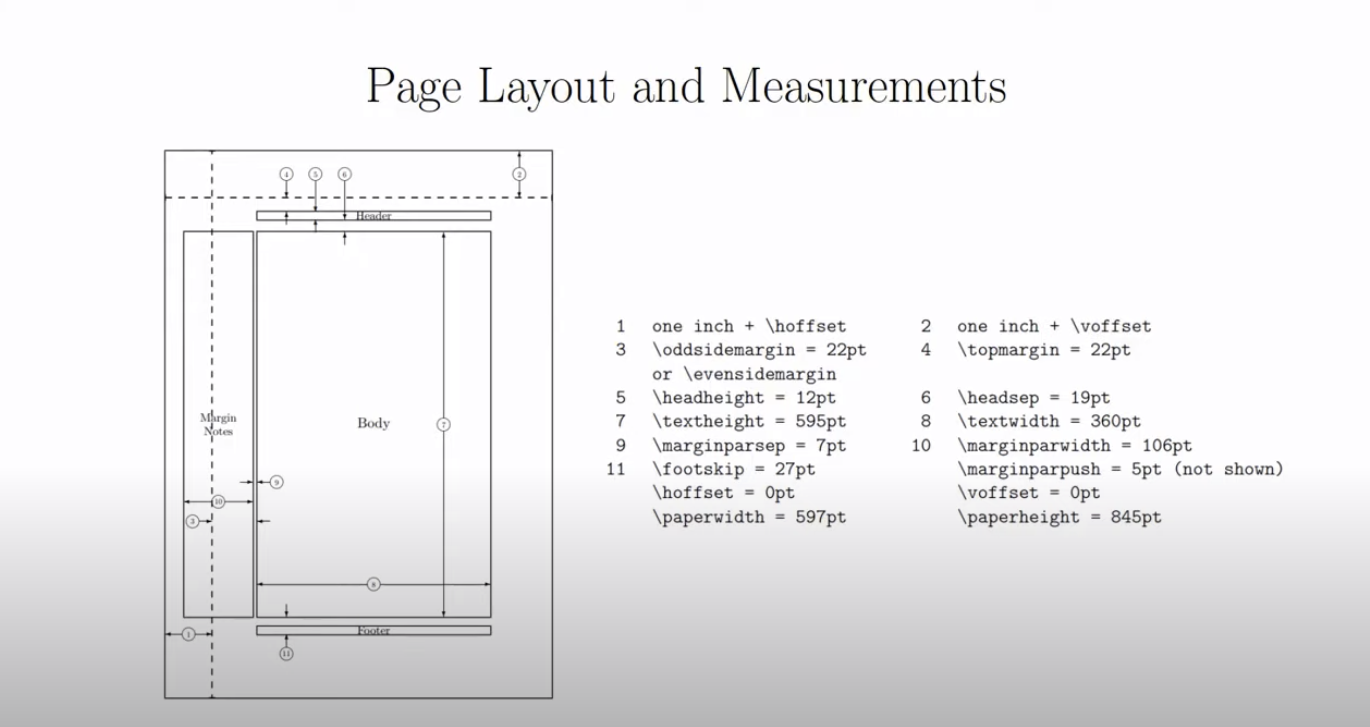
\includegraphics[width=\linewidth]{page_layout.png}
    \caption{LaTeX Page layout and Measurements (width=linewidth)}
    \label{hr_3}
\end{figure}

\section{Section with subsections}

\subsection{LARGE text}
{\LARGE \indent Nisi qui culpa pariatur velit deserunt nulla nulla dolor cillum est do nulla ut. Nisi qui culpa pariatur velit deserunt nulla nulla dolor cillum est do nulla ut.}

\subsection{huge text with bold, italic and standard underline}
{\huge \indent Nisi qui \textbf{culpa} \textit{pariatur} \underline{velit deserunt} nulla nulla dolor cillum est do nulla ut.} \\

\subsection{Huge text with combined bold, italic and standard underline}
{\Huge \indent Nisi qui culpa pariatur velit deserunt \underline{\textbf{\textit{nulla dolor cillum est}}} do nulla ut.} \\

\subsection{This is what happens when you underline long text}
\underline{\textbf{Unerlining a long string of text is kinda hard in latex with the default underline so we can use ulem}. Nisi qui culpa pariatur velit deserunt nulla nulla dolor cillum est do nulla ut. Nisi qui culpa pariatur velit deserunt nulla nulla dolor cillum est do nulla ut.} \\

\subsection{We can fix the above problem with the package ulem using uline}
\uline{\textbf{Same with ulem}. Nisi qui culpa pariatur velit deserunt nulla nulla dolor cillum est do nulla ut. Nisi qui culpa pariatur velit deserunt nulla nulla dolor cillum est do nulla ut.}

{\large \noindent ulem also has \uuline{some other} cool \uwave{underlines}.}

\subsection{Line fills and rules}

\noindent \hrulefill

\noindent Some text before fill \hrulefill

\noindent Fill by dots \dotfill

\noindent Rule can create more customizeable lines:

\noindent \rule{\linewidth}{0.4pt}

\begin{center}
    \rule{5cm}{0.4cm}
\end{center}

\subfile{sections/citations.tex}

\subsection{References to labels}

This number will take you to the specified label - \ref{eq:PythogoreanTheorem}

\noindent It can also be done as a hyperlink - \hyperref[eq:PythogoreanTheorem]{Any Custom Lable Can Be A Hyperlink}

\noindent The href command can be used for URL redirection - \href{https://example.com/}{This link will go to example.com}

\subsection{Enumeration and listing}

\begin{enumerate}[label=\arabic*]
    \item First Item
    \item Second Item
    \begin{enumerate}[label=\arabic*]
        \item First Sub Item
        \item[$\rightarrow$] Custom label
        \item Second Sub Item
    \end{enumerate}
    \item Third Item
\end{enumerate}

\begin{itemize}
    \item First Item
    \item Second Item
    \begin{itemize}
        \item First Sub Item
        \item[$\rightarrow$] Custom label
        \item Second Sub Item
    \end{itemize}
    \item Third Item
\end{itemize}

\section{Basic Math Equations}

\subsection{Displaystyle math equation}

\begin{equation} % equivalent to $$ .. $$
    \sum_{n=1}^\infty \frac{1}{n^2} = \frac{\pi^2}{6}
\end{equation}

\subsection{Inline math with display style mode}

Ex qui anim eu consequat est excepteur ea est. Exercitation officia pariatur pariatur nostrud. Cillum cillum proident minim officia ex. Aliquip ut officia sit voluptate quis dolor sint proident tempor aliquip qui enim. $ \displaystyle \sum_{n=1}^\infty \frac{1}{n^2} = \frac{\pi^2}{6} $ Elit veniam minim commodo proident do aliqua Lorem sunt ex dolore. Irure adipisicing enim eu velit eiusmod reprehenderit. Sit exercitation minim sunt et.

\subsection{Inline math with text style mode}

Ex qui anim eu consequat est excepteur ea est. Exercitation officia pariatur pariatur nostrud. Cillum cillum proident minim officia ex. Aliquip ut officia sit voluptate quis dolor sint proident tempor aliquip qui enim. $ \textstyle \sum_{n=1}^\infty \frac{1}{n^2} = \frac{\pi^2}{6} $ Elit veniam minim commodo proident do aliqua Lorem sunt ex dolore. Irure adipisicing enim eu velit eiusmod reprehenderit. Sit exercitation minim sunt et.

\subsection{Brakets sizes}

These are a bit unreadable:
\begin{equation*}
    ( \sum_{n=0}^N ( \frac{1}{a + b} )^2 )^2
\end{equation*}

\noindent We can use left and right braket:
\begin{equation*}
    \left( \sum_{n=0}^N \left( \frac{1}{a + b} \right)^2 \right)^2
\end{equation*}

\subsection{Substaking}

\begin{equation*}
    \sum_{\substack{n=0 \\ n \text{ odd}}}^\infty a_{n} x^n
\end{equation*}

\begin{equation*}
    \textstyle
    \sum_{\substack{n=0 \\ n \text{ odd}}}^\infty a_{n} x^n
\end{equation*}

\subsection{Spaces in equations}

\begin{align*}
    \int f(x) \mathrm{d}x \\
    \int f(x) \, \mathrm{d}x \\
    \iiint f(x,y,z) \mathrm{d}x \mathrm{d}y \mathrm{d}z \\
    \iiint f(x,y,z) \, \mathrm{d}x \, \mathrm{d}y \, \mathrm{d}z \\
\end{align*}

Spacing Commands:
\begin{equation*}
    \begin{array}{c c c c c}
        f(x) \mathrm{d}x & f(x) \, \mathrm{d}x & f(x) \: \mathrm{d}x & f(x) \; \mathrm{d}x & f(x) \quad \mathrm{d}x \\
    \end{array}
\end{equation*}

Using \textbf{hspace} and text to handle simple spacing issues:
\begin{equation*}
    x = 1000 \text{\hspace{1cm} and \hspace{1cm}} y = 200
\end{equation*}

\subsection{Vectors}

Vectors use the esvect package:
\begin{equation*}
    \vv{\mathrm{proj}} \quad \vv{v_1} \quad \vv*{v}{1}
\end{equation*}

\subsection{Radicals}

\begin{center}
If $ ax^2 + bx + c = 0 $ then $ \displaystyle x = \frac{-b \pm \sqrt{b^2 - 4ac}}{2a} $
\end{center}

\begin{equation*}
    \begin{array}{c c c}
        \displaystyle \sqrt[10]{\frac{1}{2}} &
        \displaystyle \sqrt[\sqrt{7}]{\frac{\sqrt[3]{\sqrt[8]{1+2}}}{\sqrt{12x}}} &
        \displaystyle \left( \sqrt[7^{\sqrt{908}}]{12}^{\sqrt[2]{8}^{\sqrt{\frac{2}{1721}}}} \right)^7 \\
    \end{array}
\end{equation*}

\section{Negation}

Build-in negations:
\begin{align*}
    a &\neq b \\
    a &\ngtr b \\
    a &\nless b \\
    a &\ngeq b \\
    a &\nleq b \\
    a &\not \approx b \\
    P &\not \implies Q \\
\end{align*}

\noindent For negation of symbols that do not have negation by default we can use \textbf{\textbackslash usepackage\{centernot\}}:
\begin{align*}
    a &\centernot \approx b \\
    P &\centernot \implies Q \\
\end{align*}

\section{Overset and Underset}

\begin{equation*}
    \begin{array}{c c c}
        a \overset{?}{=} b &
        f(x) \underset{x \to \infty}{\longrightarrow} 0 &
        f(x) \overset{?}{\underset{x \to \infty}{\longrightarrow}} 0
    \end{array}
\end{equation*}

\subsection{Theorems}

\begin{thm}[The Pythogorean Theorem] \label{eq:PythogoreanTheorem}
    $$ a^2 + b^2 = c^2 $$
\end{thm}

\begin{lem}
    $$  a = b, b = a $$
\end{lem}

\begin{defn}
    $$ \forall \mathrm{A}: \varnothing \subseteq \mathrm{A} $$
\end{defn}

\section{System of equations}

\noindent Еxample with \textbf{\textbackslash package\{systeme\}}:

\begin{equation*}
    \systeme{
        3x_{3} = 9,
        x_{1} + 5x_{2} - 2x_{3} = 2,
        \frac{1}{3}x_{1} + 2x_{2} = 3
    }
\end{equation*}

\begin{equation*}
    \sysdelim..\systeme{
        \frac{1}{3}x_{1} + 2x_{2} = 3,
        x_{1} + 5x_{2} - 2x_{3} = 2,
        3x_{3} = 9
    }
\end{equation*}

\begin{equation*}
    \sysdelim..\systeme{
        x + y = 0@p_{*},
        2x - y + 3z = 3,
        x - 2y - z = 3
    }
\end{equation*}

\begin{equation*}
    \sysautonum{L’_{*}\longleftarrow}
    \sysdelim..\systeme{
        x+y-z=3@L_1,
        3x+2y=7@L_1+L_2,
        3x+y=6@2L_1+L_3
    }
\end{equation*}

\begin{equation*}
    \sysautonum*{L_{*}}
    \systeme{a+b=4, 2a-b=5}
    \quad
    \systeme{x-3y=0, 2x+y=1}
\end{equation*}

\begin{equation*}
    \sysdelim..\systeme{
        x_{1} + 6x_{2} = 9,
        - x_{2} - 2x_{3} = -7,
        x_{3} = 3
    }
    \quad
    \longrightarrow
    \quad
    \sysdelim..\systeme{
        x_{1} + 6x_{2} = 9,
        x_{2} = 1,
        x_{3} = 3
    }
    \quad
    \longrightarrow
    \quad
    \sysdelim..\systeme{
        x_{1} = 3,
        x_{2} = 1,
        x_{3} = 3
    }
    \end{equation*}

Systems can be aligned in specific order [tzxy]:

\begin{equation*}
\systeme[tzxy]{
    x+2y-3z+t=0,
    2x-y-z+3t=4,
    2y+3z+4t=-1,
    3x-2z-2t=3
}
\end{equation*}

\section{Tables}

\subsection{Simple Tables}

\begin{tabular}{lcr}
    left justified & centered & right justified \\
    l & c & r
\end{tabular}

\noindent Table with boarders \\

\noindent
\begin{tabular}{ | l |c r| }
    \hline
    left justified & centered & right justified \\
    \hline
    l & c & r \\
    \hline
\end{tabular}

\noindent Note that begin center is quite limited for tables, but can work for a quick and simple solution sometimes: \\
\begin{center}
    \begin{tabular}{ | l |c r| }
        \hhline{ | - | - | - | }
        left justified & centered & right justified \\
        \hhline{ | - | ~ - | }
        l & c & r \\
        \hhline{ | - | ~ - | }
    \end{tabular}
\end{center}

\subsection{Long text in column and other table packages}

This problem: \\
\begin{tabular}{ | l | c | r | }
    \hline
    long text in table long text in table long text in table long text in table long text in table long text in table long text in table long text in table long text in table &
    long text in table long text in table long text in table long text in table long text in table long text in table long text in table long text in table long text in table &
    long text in table long text in table long text in table long text in table long text in table long text in table long text in table long text in table long text in table
    \\
    \hline
\end{tabular}

\noindent Can be fixed like this, with 3 custom commands defined in the preamble:

\begin{tabular}{ | L{5cm} | C{4cm} | R{3cm} | L{4cm} | }
    \hline
    For more advanced tables we can use the \textbf{\textbackslash usepackage\{booktabs\}} - Provides extra commands to make tables more attractive &
    For more advanced tables we can use \textbf{\textbackslash usepackage\{tabularx\}}, which provides another way to control the width of the columns &
    For more advanced tables we can use \textbf{\textbackslash usepackage\{colortbl\}} to add color to tables, including line colors and cell background colors &
    For more advanced tables we can use \textbf{\textbackslash usepackage\{longtable\}} for large tables that span across multiple pages
    \\
    \hline
\end{tabular}

\subsection{Multi-column tables}

\begin{tabular}{ | C{3cm} | C{3cm} | C{3cm} | }
    \hline
    Magna excepteur occaecat culpa voluptate & incididunt officia irure cupidatat & eiusmod consequat ut occaecat anim consectetur. \\
    \hline
    \multicolumn{3}{ | R{9cm} | }{Proident in culpa consequat fugiat.Anim dolor exercitation voluptate irure exercitation adipisicing proident veniam incididunt sit sunt.} \\
    \hline
    Testing & \multicolumn{2}{ | L{6cm} | }{Laborum sit aliquip laborum commodo cupidatat.Exercitation fugiat dolore fugiat Lorem sit non enim.Pariatur nulla nulla non ullamco adipisicing velit.} \\
    \hline
\end{tabular}

\section{Multi-row tables}

We can use the command
\begin{verbatim} \multirow[vertical_aligment]{num_rows}{width}{content} \end{verbatim}

\begin{center}
    \begin{tabular}{ c c }
        \multirow[c]{2}{*}{Row Merge} & Text \\
        & Text \\
    \end{tabular}
\end{center}

Advanced multi-row example:
\begin{center}
    \renewcommand\arraystretch{1.3}
    \begin{tabular}{|c|c|c|c|c|}
     \hline
     Text A     & Text B    & Text C    & Text D    & Text E    \\
     \hline
     A          & Text F    & Text G    & Text H    & Text I    \\
     \hline
     B          & Text J    & Text K    & Text L    & Text M    \\
     \hline
     \multirow{3}*{Text N}
                & \multirow{3}*{Text O}
                            & Text P    & Text Q    & Text R    \\
     \cline{3-5}
                &           & \multirow{2}*{Text S}
                                        & Text T    & Text U    \\
     \cline{4-5}
                &           &           & Text V    & Text Z    \\
    \hline
    \end{tabular}
\end{center}

\section{Arrays}

\subsection{Simple Arrays}

Arrays are usually used for matrices:
\begin{equation*}
    \left[
        \begin{array}{ ccc }
            a_{11} & a_{12} & a_{13} \\
            a_{21} & a_{22} & a_{23}
        \end{array}
    \right]
\end{equation*}

\noindent But it's easier and more versatile to use \textbf{pmatrix}, \textbf{bmatrix}, or some others from the \textbf{amsmath} package: \\
\begin{equation*}
    A_{m,n} =
    \begin{pmatrix}
    a_{1,1} & a_{1,2} & \cdots & a_{1,n} \\
    a_{2,1} & a_{2,2} & \cdots & a_{2,n} \\
    \vdots  & \vdots  & \ddots & \vdots  \\
    a_{m,1} & a_{m,2} & \cdots & a_{m,n}
    \end{pmatrix}
\end{equation*}
\begin{equation*}
    B =
    \begin{bmatrix}
    a & b & c \\
    d & e & f \\
    g & h & i
    \end{bmatrix}
\end{equation*}
\begin{equation*}
    \begin{Bmatrix}
    a_{11} & a_{12} & a_{13}  \\
    a_{21} & a_{22} & a_{23}  \\
    a_{31} & a_{32} & a_{33}  \\
    \end{Bmatrix}
\end{equation*}
\begin{equation*}
    \overrightarrow{v} = \left(\begin{array}{ c }1 \\ 2 \\ 3\end{array}\right)
\end{equation*}

\section{Formatting code}

The simplest way to fromat code is to use verbatim:
\begin{verbatim}
    a := int32(0)
    for i := 0; i < a; i++ {
        fmt.Println(i)
    }
\end{verbatim}

\noindent More advanced way is with \textbf{\textbackslash usepackage\{minted\}} witch has some level of syntax highlighting:
\begin{minted}{go}
    type Client struct {
        rawConn *limitconn.Wrapper
        handshake *clientHandshake
    }

    func (c *Client) Connect(ipv4 string, port uint16) error {
        addrss := fmt.Sprintf("%s:%d", ipv4, port)
        conn, err := net.Dial("tcp", addrss)
        if err != nil {
            return err
        }

        fmt.Printf("client connection on %d\n", port)
        c.rawConn = limitconn.Wrap(conn, "client_"+rand.GenString(32))
        c.rawConn.SetLimit(clientHandshakeLimit)
        c.handshake = NewClientHandshake(c.rawConn)
        if err := c.handshake.Handshake(); err != nil {
            c.rawConn.Close()
            return err
        }

        return nil
    }
\end{minted}

\noindent If needed, the minted package can also load snippets from files!

% BIB:
\newpage
\printbibliography

\end{document}